\documentclass{article}
\usepackage[UTF8]{ctex}

% Language setting
% Replace `english' with e.g. `spanish' to change the document language
\usepackage[chinese]{babel}

% Set page size and margins
% Replace `letterpaper' with `a4paper' for UK/EU standard size
\usepackage[a4paper,top=2cm,bottom=2cm,left=3cm,right=3cm,marginparwidth=1.75cm]{geometry}

% Useful packages
\usepackage{amsmath}
\usepackage{graphicx}
\usepackage[colorlinks=true, allcolors=blue]{hyperref}

\title{基于改进遗传算法的无人仓多 AGV 防碰撞的路径规划研究}
\author{王宏坤、陈屹安、刘熠}

\begin{document}
\maketitle


\section{摘要}

	针对无人仓的多搬运机器人的路径规划问题,我们构建了线性规划模型,综合运用了遗传算法和退火算法等方法, 并借助 python、c++、matlab编程求解。
	
	首先我们对给出的数据进行数据预处理:(1)由题目所给的map.csv文件,我们通过python,把地图的每个坐标节点抽象为顶点,可连通的顶点直接连线,运用networkX第三方库构建了无向图。 (2)根据无向图,我们采用了floyd算法得出了各节点直接的邻接矩阵和路由矩阵,并对无向图进行了可视化。(3)根据agv.csv,我们把AGV画在了地图中,并删除了不合理的数据,正常的AGV共有19个。
	
	
对于问题一, 本题要求满足以下约束: 1)AGV只能横向、纵向移动,不可斜向移动。 2)order.csv文件中的所有订单全部满足 3)拣选工位只能同时存放b个托盘(本题中我们不妨假设b等于3)。 
 根据题意, 我们将构建单目标规划模型, 基于托盘搬运顺序进行编码, 并采用改进的遗传算法和模拟退火两种方法进行对比求解。 通过改进的遗传算法求解后可以得到, 所有 AGV 的路径总长度为 7316; 通过模拟退火算法求解后可以得到所有 AGV 的路径总长度为 7428。 通过两种方式的比较, 可以得到改进遗传算法使得 AGV 以更短的路径搬运完所需要的商品
 
 
 
 
 \textbf{关键词} 遗传算法 退火算法 floyd算法
 
\section{问题重述与分析}

\subsection{问题背景}
随着电商的兴起, 无人仓逐渐作为自动化仓储物流系统的发展方向和目标。 仓库管理(也叫仓储管理)是对仓库内货物的接收、 存储、 发货等一系列活动进行有效的控制管理, 维护仓库货物并确保日常经营活动正常进行。 传统的仓库管理模式大多是人工管理模式, 而这种管理方式有着不少问题, 特别是因为人力效率低下的因素导致的“爆仓”现象。 最早的包括 Amazon 的 Kiva 机器人, 以及后来 AGV 搬运机器人、 SHUTTLE货架穿梭车、 DELTA 分拣机器人等各式各样的、 高度自动化的机器人都是为仓库的无人化量身定制的。 而无人仓内搬运机器人的调度问题是其中的核心问题。在对问题进行分析之前, 首先要了解一下概念。(1) 搬运机器人, Automated GuidedVehicle (AGV), 通过特殊地标导航自动将物品运输至指定地点。 它是执行仓库内任务的主要单元, 可以通过指令指派一个 AGV 去取一个货架到仓库内指定地点, 比如拣选工位, 储位, 回收处等; (2) 托盘和储位。 仓库内绝大部分区域都是放置托盘的储位, 而托盘上摆放着待出库商品。 有的仓库里托盘用多层的货架代替, 无论货架还是托盘都可以被 AGV 搬运; (3) 拣选工位。 由分拣机器人拣选商品, 完成打包后通过传送带输送出库, 包括了多个放置托盘的停靠位, 分拣机器人以及商品出库的传送带; (4) 托盘回收处。 仓库内用来回收空托盘的固定区域, 一般仓库内会指定 2-4 个固定位置为托盘回收处。

\subsection{问题一}
对于问题一,假设不考虑小车的可能的碰撞问题,在无人仓的模型下设计调度,根据附件中的订单数据,仓库中的库存数据,使得每个小车尽可能忙的同时,最小化的行走总路径。

\subsection{How to include Figures}



\begin{figure}
\centering
\includegraphics[width=0.50\linewidth]{mapAGV.png}
\caption{\label{fig:frog}}
\end{figure}

\begin{figure}
	\centering
	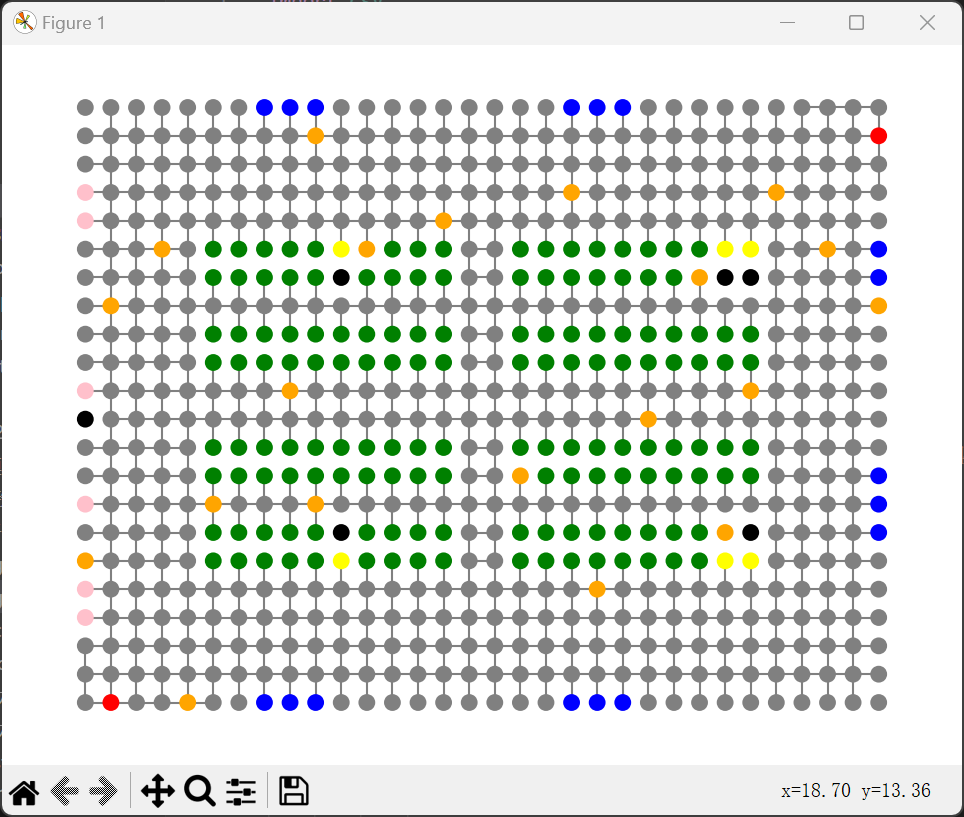
\includegraphics[width=0.50\linewidth]{map.png}
	\caption{\label{}}
\end{figure}

\subsection{How to add Tables}


\section{基本假设}
假设一:刚开始可正常运行的小车不会因内部原因发生故障

假设二:所有小车任何情况下速度相同且为一

假设三:每个小车占据大小刚好为一个栅格

假设四:拣选工位,存储仓位可以让小车通过

假设五:所有小车相撞对其运行无影响(仅对问题一、问题二适用)假设六:每个拣选工位的拣选商品速度相同(仅对问题一、问题二适用)

假设七:每次小车在拣货完成后都回到此次任务的托盘节点,简化了回库与回收问题。

假设八:对于 b 个停靠点的约束,我们在第一问中假设为无穷大,忽略 b 个停靠点对问题造成的影响。
\bibliographystyle{alpha}
\bibliography{sample}

\section{符号说明}


\begin{tabular}{l|r}
		\centering
		符号 & 相关意义 \\\hline
		$EMPTY_i$ & 表示空储位节点的坐标的集合 \\
		$GREEN_i$ & 表示所有储位节点的坐标集合,上面放置了托盘\\
		$QUANTITY_i$ & 表示$green_i$上含有的商品\\
		$BLUE_i$ & 表示拣选工位节点的坐标集合,即Agv从储位节点取出托盘后的目的地\\
		$RED$ & 表示所有空托盘回收节点\\
		$D_i$ & 表示$green_i$上的托盘在某次Agv的出库回库(出库回收)任务中经过整条完整路径的长度\\
		$DE_{empty_i}$ & 表示回库任务过程中空储位节点$empty_i$到最近拣选工位的距离\\
		$YX_{green_i,blue_j}$ & 表示某次Agv搬运$green_i$的托盘过程中要优先选择哪个拣选工位节点$blue_i$\\
		g(i) & 表示第i次搬运过程中搬运的托盘编号($green_i$)\\
		$DIS_{ij}$ & 距离矩阵\\
		$ADJ_{ij}$ & 邻接矩阵\\
		$ROU_{ij}$ & 路由矩阵\\
\end{tabular}


\section{问题分析}
\subsection{问题一}
问题一要求我们在不考虑 AGV 之间的碰撞体积和拥堵情况的前提下对 AGV 的路程进行最小化,首先,由于有一个 AGV 故障,排除在外,同时考虑使用蚁群算法进行路径优化和实现避障功能,又考虑到有可能会出现多个 AGV 前往同一个储位节点而造成路程浪费和不必要的拥堵,为了避免此类问题发生,希望通过先到先得的思想,将 AGV 进行编号,给每个 AGV 分配不同的储位节点,同时使用遗传算法综合考虑所有可能产生的路程长度,求出所有可能性的最小值,即最小的路程长度,在全场 AGV 的速度保持不变的前提下,即为相对的全局最优解

\subsubsection{问题一模型建立}

为了方便进行统计和计算,我们定义一个函数f(x)来判断某个$green_i$的托盘是否需要进行搬运



对于$x\in C$,若x≠0,则$f(x)=1$;否则$f(x)=0$.若x为矩阵,则对x中的每个单独元素$x_i$使用f函数

(我们用$f(d_{green_i})=1$来表示某个$green_i$的托盘需要进行搬运)

先暂时不考虑后续目标规划时使用的算法,我们建立本题的目标规划模型如下:

记所求的答案为Z,表示所有Agv进行的路程总和的最小值,因为当所有商品拣选完成就代表结束,所以我们有
$Z=min({Green}^TD+M^TD')①$

即正常运输的agv的路程+补货的路程(的最小值)

考虑约束条件“满足所有订单需求”,我们有以下方程:
$
(\sum_{i=1}^{n} {quantity_{green_i}*f(D_{green_i})})+M-QUANTITY_{需求}≥0②$

注:这里$(\sum_{i=1}^{n} {quantity_{green_i}*f(D_{green_i})})$表示一个集合,按商品SKU顺序记录所有搬运托盘的商品库存总和,下同
考虑约束条件“实现Agv尽可能忙”,我们有以下方程:

我们用集合$\Delta$ t表示第t次搬运某个托盘经过拣选后剩余商品的情况,
$\Delta$ $t=QUANTITY_{需求}-(\sum_{i=1}^{t-1}$ ${quantity_{green_{g(i)}}*f(D_{green_{g(i)}})}+QUANTITY_{green_{g(t)}})③$
注:这里的$\Delta t$中$QUANTITY_{需求}$矩阵暂时只考虑托盘上含有的商品所对应行

这里,$f(\Delta t)=1$表示托盘还有剩余商品,$f(\Delta t)=0$表示该托盘已经为空托盘

我们新定义一个矩阵$DISS=(DISS_{green_i,blue_j})^T$,表示某次Agv从$green_i$搬运到拣选工位节点$blue_j$一次工作

周期的完整路程长度(包含了回库和回收过程)且最短,这里有$$D_{green_i}=DISS_{green_i,blue_j}④$$

要计算这个“完整路径长度”,我们有:
$$DISS_{green_{g(t)},blue_j}=dis_{green_{g(t)},blue_j}+f(\Delta t)*(dis_{blue_j,empty_k}+dis_{empty_{k},green_{g(t+1)}})+(1-f(\Delta t))*(dis_{blue_j,red_l}+dis_{red_l,green(t+1)})⑤
$$


由于我们说的“每一次完整路径”都从agv从$green_i$搬运托盘开始,所以一条路径也应从agv到(另)一个$green_j$结束

所以我们需考虑$dis_{empty_k,green_{g(t+1)}}$等几项。这里,在第t次搬运中,$dis_{green_i,blue_j}$表示$green_i到blue_j$的最短路程

$f(\Delta t)*dis_{blue_j,empty_{g(t)}}$表示当托盘拣选后非空,该托盘被Agv带回库的最短路径长,即$DE_{empty_{g(t)}}$
$$(1-f(\Delta t))*dis_{blue_j,red_k}$$表示当托盘经拣选后为空托盘时被Agv回收的最短路径长

$f(\Delta t)*dis_{empty_k,green_{g(t+1)}}$表示当托盘非空时,agv把托盘运至空储位节点后到
$green_{g(t+1)}$下一次搬运托盘的距离
$$(1-f(\Delta t)) \times (dis_{blue_j,red_l} + dis_{red_l,green_{t+1}})$$
表示当托盘为空时,agv把托盘运输到$red_l$回收后到$green_{g(t+1)}$下一次搬运托盘的距离考虑约束条件“每个拣选工位尽可能忙”,我们需要确定搬运的优先级,有:
$$YX_{green_i,blue_j}+DISS_{green_i,blue_j}≤YX_{green_i,blue_k}+DISS_{green_i,blue_k}$$,
其中,$$BLUE_j\in BLUE,\forall blue_k\in BLUE⑥$$
(这也符合了我们对集合D“最短”的定义)结合①②③④⑤⑥,我们建立数学模型并可以进一步使用计算机求解。

\subsubsection{问题一改进遗传算法和模拟退火算法设计}
本题属于NP Hard问题,若采用枚举算法求解,时间呈指数级增长,陷入灾难级别的计算量,故我们将采取遗传+退火的现代优化算法,尝试找到一个局部最优解。
	
	遗传算法的实现过程主要通过对问题的每一个参数进行编码, 并产生初始种群, 计算适应度, 然后进行复制、 交叉、 变异, 如此循环往复 N 代, 产生最优的子代, 以此确定为全局的最优解。 
	
	\textbf{步骤一: 融入“储位节点搬运判别要素” 的基因编码}
	
	
	
	我们的编码方式是:创建19个字典,每个字典的索引为各储位节点的id,各索引的值为0或1(其中0代表未访问,1代表访问),从而我们构建了19个分别代表各AGV行走路线的编码,即染色体。如{001:1|002:0|003:0| ······ 019:1}。
	
	\textbf{步骤二: 初始种群生成}
	
	我们采用python生成随机数的方法生成了200个可行解,选择步骤三中适应度最高的方案,作为初始种群
	
	\textbf{步骤三: 适应度设计}
	
	选择亦称再生或复制, 选择过程是个体按照其适应度进行择优复制。 在本题中我们将目标函数值认定为适应度函数 fitness。 按照适应度概率挑选优秀的子代进行复制, 淘汰效果不佳的子代, 以便于之后的子代都普遍更接近于最优值。 其中我们往往通过随机方法来实现选择的操作. 因本题具体计算的基因长度过长, 故我们基于上述编码中的例子示意, 我们的选择过程如下:
	$$(1-f(\Delta t)) \times (dis_{blue_j,red_l} + dis_{red_l,green_{t+1}})$$
	表示当托盘为空时,agv把托盘运输到$red_l$回收后到$green_{g(t+1)}$下一次搬运托盘的距离考虑约束条件“每个拣选工位尽可能忙”,我们需要确定搬运的优先级,有:
	$$YX_{green_i,blue_j}+DISS_{green_i,blue_j}≤YX_{green_i,blue_k}+DISS_{green_i,blue_k}$$,
	其中,$$BLUE_j\in BLUE,\forall blue_k\in BLUE⑥$$
	
	\textbf{步骤四: 交叉算子设计}
	
	为了创建一对新个体,通常将从当前代中选择的双亲样本的部分染色体互换(交叉),以创建代表后代的两个新染色体。此操作称为交叉或重组。由于初始种群已是可行解,故交叉以后只是改变了完成订单的AGV,因此交叉以后的依然为可行解。
	
	我们用python随机抽取交叉节点和交叉染色体
	\begin{figure}GA
		\centering
		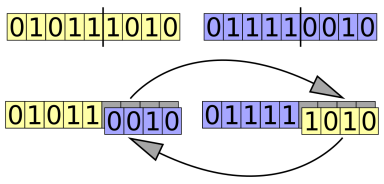
\includegraphics[]{GA1.png}
	\end{figure}
	
	
	\textbf{步骤五: 变异算子设计}
	
	
	同时我们规定变异概率$P_i$以式(3-8) 自适应的方式得到, 从而保证当种群中的个体适应度值趋于一致时, 则会增加变异运算的概率, 当个体适应度值趋于分散的时候,则减小变异运算的概率。 并且该方法使得适应度高的个体对应变异的概率减小, 适应度低的个体对应变异概率增大, 有助于保护高适应性的个体, 淘汰低适应性的个体, 能够更好地找到最优解。
	
	\subsubsection{问题一的求解}
本题基于上述的模型与遗传算法, 通过 Python 语言进行编程实现, 最终计算结果为: 所有搬运机器人的总路径为 8248
\begin{figure}

	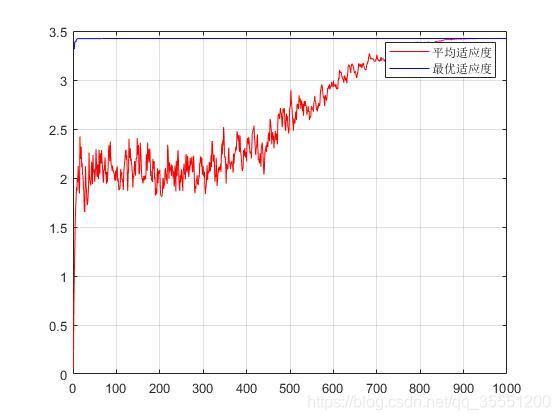
\includegraphics[width=0.50\linewidth]{Solution1.jpg}
	\caption{\label{}}
\end{figure}
\begin{figure}

	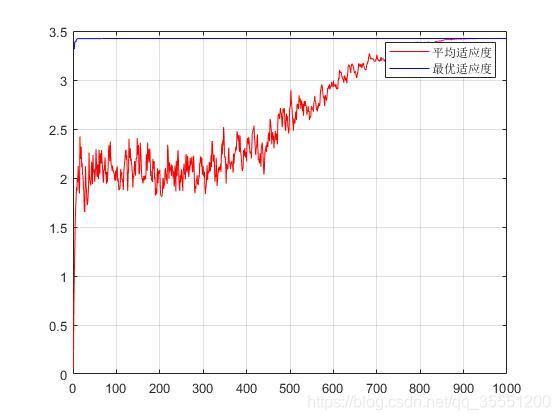
\includegraphics[width=0.50\linewidth]{Solution1.jpg}
	\caption{\label{}}
\end{figure}
	\begin{figure}
		\centering
		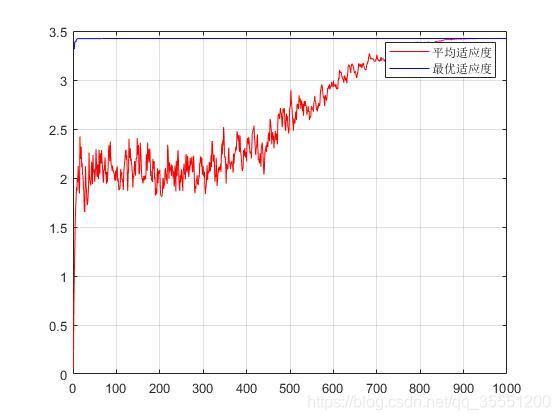
\includegraphics[width=0.50\linewidth]{Solution1.jpg}
		\caption{\label{}}
	\end{figure}
	
\end{document}




